\documentclass{cshonours}

\usepackage{url}
\usepackage{minted}
\usepackage{graphicx}
\usepackage{pdflscape}
\usepackage[style=alphabetic, sorting=nyt]{biblatex}
\addbibresource{bibliography.bib}

\title{6CCS3PRJ \\\vspace{0.5cm}
  A Pragmatic Infrastructure Modelling and Verification Framework}
\author{Joe Stanton\\\vspace{0.5cm}
  Student ID: 1020836
}

\begin{document}

\maketitle

\chapter*{Abstract}
The complexity of software and the scale at which services must operate is continuing to increase rapidly~\cite{SoftwareComplexity}.
To support this rapid growth, the supporting application infrastructure needed to keep these services running and providing a suitable quality of service must grow proportionally.

A typical stack for delivering scalable web based applications now consists of many interconnected parts, including database servers, application servers, caching layers, load balancers and network hardware.
This inevitable growth in both application and infrastructure complexity presents significant engineering challenges in the design of fault-tolerant and performant distributed systems.

While the problems of delivering software at scale are significantly reduced by the cloud computing movement, the inherent complexities of distributed systems with many components and therefore points of failure continually prove to be problematic. Infrastructure complexity is steadily increasing, and is a leading cause of downtime and unreliability. According to a recent Gartner survey, 73\% of IT executives say their infrastructure complexity is either `high' or `out of control'~\cite{Gartner2013}. Managing this complexity, and therefore being able to efficiently identify and fix issues is the key to providing the reliable and performant services we expect, over time.

In this report, we discuss and implement an infrastructure modelling and monitoring tool that can be used to help manage some of the inherent complexity in modern infrastructure. The emphasis of this investigation is on small to medium size software deployments, rather than enterprises that typically have the resources to tackle these problems.

\chapter*{Originality Avowal}
I verify that I am the sole author of this report, except where explicitly stated to the contrary. 

\textbf{Signed:} Joe Stanton 

\textbf{Date:} \today

% \chapter*{Acknowledgements}

\tableofcontents

\chapter{Introduction}

\section{Thesis}
\textit{It is practical and useful to develop an infrastructure modelling and monitoring tool to help address the inherent complexity in modern IT infrastructure.}
\section{Motivation}

After taking part in the delivery of software in the highly regulated insurance industry, I noted some problems with the reliability of the software delivered. These reliability issues were generally unrelated to the application itself, but predominantly caused by the growth in complexity of the underlying application infrastructure, which was provided and managed within the company's own datacenter as a result of regulatory constraints. As the application grew in complexity over time, the number of dependent services and components needed to keep it running became unmanagable by the company's own IT staff.

I discovered a real disparity between the knowledge application developers had of the specific requirements of their application (hardware specifications, dependencies on other services, likely points of failure) and the lack of awareness of this within the operations team. This phenomenon has been noted in other areas of the industry~\cite{DevOps} and has recently given rise to the term `DevOps' - an attempt to improve communication between the teams or build tools which help to do so.

Better collaboration and knowledge transfer between these teams often provides the following benefits:

\begin{description}
  \item [Proactive maintenance of the system and its dependencies]\hfill \\
    The effect of changes is well understood by all members of the team and problems can be foreseen ahead of time. The infrastructure can be modernised progressively.
  \item [Identification of weaknesses in the system architecture]\hfill \\
    e.g.\ single points of failure, overworked or repeatedly unreliable components can be identified, and discussion between the teams can lead to effective solutions.

  \item [Reduced risk of change]\hfill \\
    Delivery of features and bug-fixes to deployed software can happen regularly and reliably through Continuous Delivery.

  \item [Quick and effective root cause analysis]\hfill \\
    When issues do occur, they can be diagnosed and fixed quickly, and then prevented in the future.
\end{description}

\section{Solution Objectives}

The objective is to design and implement a tool which helps with the modelling of complex infrastructure within real-world systems. The application will provide application developers or operations staff the ability to model systems as a graph of nodes, which may have dependencies and fine grained tests used to verify their current state.

The tool will then execute this model as a means of system monitoring. It will verify the correctness of the live system continuously and warn of any divergence. It will also allow the attachment of metadata and metrics to nodes. This model, metadata and metrics will then serve as a useful diagnostic tool if the state of the system changes, e.g.\ a loss of connectivity between two nodes. This fine-grained and clear mechanism of communicating failure should reduce investigation and response times when issues arise, and provide the insight which prevents them from recurring.

This model can serve as `living documentation' which is used by Ops teams and Developers to help manage and transfer knowledge, documenting their implicit knowledge. It should help to predict the impact of changes. It should improve collaboration between the teams and provide deeper insight into issues with the performance or reliability of the system.

Languages and tools for the modelling of software architecture and infrastructure do exist, however they lack the simplicity and pragmatism in their implementation to see widespread adoption in industry~\cite{ModellingAdoption}. I propose a simple, pragmatic tool which may come with some modelling limitations, but will be quick and easy to set up and begin reaping the benefits.

Given its role as the centralised location of knowledge for the system, this tool could become a platform to solve other distributed systems issues, such as service discovery etc.\ but these problems are not part of the initial scope.

\section{Software Platform and Target OS}

The system will be developed in multiple parts and distributed across hosts, where an appropriate choice of programming language will be used to suit the task. The application will generally consist of a web based modelling tool, which also provides feedback on the current state of the system, and a set of background processes that perform the verification and feed changes back to the web interface.

All user interaction will be web based, due to the ease in distributing and updating the system and the lack of an installation step. Latest browsers with HTML5 and CSS3 support will be targeted as these are common amongst IT professionals. More details on the chosen system architecture are presented in section~\ref{section:architecture}

\textbf{Scope Limitations:} Due to the significant differences between Windows and UNIX based servers, including compatibility of tools, remote command execution strategies and scriptability, I have decided to target only UNIX based (specifically Linux) servers initially. This decision is based upon the dominance of UNIX within the server market, at 66.8\% in a 2013 study~\cite{UnixMarketShare}.

\chapter{Background Research \& Literature Review}

In this chapter, we discuss the increase in infrastructure and software complexity, and how the industry has adapted to deal with it. We also review some literature from related research fields and evaluate the effectiveness of the proposed solutions.

\section{Managing Software Complexity}

The problem of increasing software complexity is a well publicised and researched phenomenon. Software which is complex takes longer to develop, and is harder to maintain. As it affects the value proposition to the user so directly, it is often the dominant factor in determinining the feasibility of implementing a given system.

The rise in software complexity together with ever changing business demands during its development has given rise to a number of popular methodologies or techniques in research and industry, such as Model Driven Development~\cite{MDD}, Extreme Programming~\cite{BeckXP} and the Agile movement~\cite{AgileManifesto}.

\subsection{Modelling and Model Driven Software Engineering (MDSE)}

Modelling of complex software has been used for a number of years as a tool of communication between developers, project managers and stakeholders. A number of tools can be used to produce clear diagrams of a system, but models provide a level of semantic meaning that allows them to be practically used to derive or verify an implementation. The Unified Modeling Language is considered the de-facto set of graphic notation techniques to create visual models of object-oriented software-intensive systems~\cite{UMLDefinition}.

\paragraph{Diagrams vs.\ Models}
A drawing tool can only be considered a modelling tool only if the tool `understands' the drawings~\cite[p.~11]{ModelDrivenDevelopment}. This has a number of benefits:

A modelling tool guarantees a minimum level of semantic meaning and model quality, because they grant alignment to some sort of meta-model~\cite[p.~12]{ModelDrivenDevelopment}.
The model can often be used to derive an implementation or perform checks/validation to ensure that a given implementation satisfies the model.


\paragraph{Modelling Techniques}
Models can be built textually as well as graphically. Textual models are commonly expressed using Domain Specific Languages (DSL’s). A DSL is defined as ``a computer programming language of limited expressiveness focused on a particular domain"~\cite{FowlerDSL}. Textual models can still sometimes be used with graphical tooling to provide a visualisation of the expressed model.

\paragraph{Adoption of Modelling and MDSE}

Studies into increased quality, maintainability and developer productivity when using MDSE techniques can be found commonly in academia but are difficult to find in industry. In a study into Industrial Adoption of Model Driven Development, it was stated that "interviewees emphasized tool immaturity, complexity and lack of usability as major barriers to adoption"~\cite{IndustryMDSE}.

\pagebreak
\subsection{Unit and Integration Testing}

The XP and Agile movements focus on improving software quality and increased responsiveness to changing customer requirements~\cite{WikiXP}. These are both process management and technological issues. XP focuses mostly on the technical aspect, there is a very strong focus on testing, and Test Driven Development (TDD) in particular which helps to realise these goals.

There are many types of testing, but they can generally be grouped into three main categories:

\begin{description}
  \item[Unit Testing] The main role of unit testing is as a design tool, developers can write unit tests to specify the intended behaviour of a component and then implement it to match. They provide fast and specific feedback on the correctness of implementation.
  \item[Integration Testing] verification that each separate component of the system functions correctly when it has been integrated with other components. This could range from testing the composition of two small components or an entire order processing pipeline. They are used to improve confidence in overall system correctness, and they are often use to guard against regressions in functionality over time.
\end{description}

Testing is often used as a means of managing complexity, especially as systems become larger. A suite of tests is often used as a means to provide quick feedback when changes break other areas of the system. We can see many similarities between the complexity of software and the complexity of its underlying infrastructure, therefore these techniques could have value in this area too.

\pagebreak
\section{Managing Infrastructure Complexity}

There is clearly a large amount of research and analysis into managing software complexity, in this section, we will review the techniques used to manage the infrastructure side of this complexity.

\subsection{General Modelling Tools}

A number of modelling standards are extremely flexible and allow the expression of arbitrary systems. One example of this is the Common Information Model (CIM) standard~\cite{CIM}. There are many IDE’s and tools that have the ability to construct CIM compliant models, such as the Eclipse Modelling Framework~\cite{EMF}.

It is relatively difficult to find practical examples of infrastructure modelling in CIM, making it difficult to get started with unless the user already has experience with MDSE techniques.

Such generic modelling tools are useful for communicating ideas or states of a system, but it could be argued that they lack pragmatic value. They are generally not  executable like their software modelling counterparts, which limits their value significantly.

\subsection{Infrastructure Modelling Tools \& Configuration Management}

Modern configuration management tools can be considered a type of infrastructure modelling tool. Most of these tools such as Puppet~\cite{Puppet}, or Chef\cite{Chef} use a Domain Specific Language to declaratively define hosts, their respective software stack, and install and manage their respective services.

Configuration management tools are especially interesting due to their mass adoption in recent years within the Agile software development community, as well as at enterprises such as Facebook and Amazon~\cite{Chef}.

The real value of these DSL's is that they are directly executable. 
They can be executed to drive infrastructure changes or ensure convergence with the model. Figure~\ref{fig:PuppetDSLSnippet} provides an example snippet of a Puppet recipe, which is declaratively specifying details of the SSH (secure shell) service which will be made available on a specific host.

\begin{listing}[h]
\begin{minted}[fontfamily=fi4]{ruby}
class sshd {
    package { 'openssh-server':
        ensure => latest
    }
    service { 'ssh':
        subscribe => File[sshdconfig],
        require   => Package['openssh-server'],
    }
    file { 'sshdconfig': 
        name    => '/etc/ssh/sshd_config',
        owner   => root,
        group   => root,
        mode    => 644,
        source  => 'puppet:///sshd/sshd_config',
        require => Package['openssh-server'],
    }
}
\end{minted}
\caption{A puppet recipe snippet, declaratively configuring the SSH service on a host. The execution of this description is idempotent, so can be repeated safely to ensure convergence.}
\label{fig:PuppetDSLSnippet}
\end{listing}

As part of the runtime execution, each service’s conformance to this set of properties is verified and if there is any divergence, the tool will orchestrate a set of imperative actions, for example installing the service or altering its configuration file and then restarting it.

\clearpage
\subsection{Existing Monitoring Tools}

I have extensively researched existing monitoring tools ranging from very simple ping checks to complete enterprise solutions and evaluated their effectiveness. In the interest of brevity, I have included a small sample of popular monitoring tools I have evaluated which give an indication of the cross-section of the market:

\subsubsection{Nagios}

Nagios is an open source infrastructure and application monitoring framework. Often considered the `industry standard', it provides a vast array of features, from execution of fine-grained protocol specific tests to complex capacity planning techniques. It is also very extensible, which is perhaps the largest reason for its success within the industry.

Nagios is in active use by over 250,000 organisations worldwide, including Amazon, AT\&T and JP Morgan Chase~\cite{NagiosUsage}. It supports a number of common montitoring architectures, including both agent based and agentless (based on the Simple Network Management Protocol) which means it can run efficiently up to a very large number of hosts~\cite{NagiosArchitectures}.

Anecdotal feedback about Nagios typically suggests that it is a mature and flexible solution for basic monitoring of large numbers of hosts, but severely lacks some higher level concepts such as integration tests of system components. It is also considered extremely time consuming and unintuitive to set up and manage, which perhaps explains its lack of adoption within smaller businesses/startups.

\subsubsection{StatsD, CollectD, Graphite}

This collection of tools all work together in providing near real-time metrics tracking and graphing, they are used heavily at vastly successful startups such as 37signals, GitHub and Shopify. Metrics can be collected from the infrastructure and application layers. 
CollectD is a system utility written in C which periodically makes system calls to extract performance fundamentals such as CPU, memory and network usage. 

Application level metrics can be collected using StatsD. Applications can send metrics to a local StatsD instance via UDP, which adds very little performance overhead. This means that it is possible to heavily instrument the critical paths of an application except in extremely performance sensitive scenarios. Both of these tools aggregate this data and flush it to a backend Graphite instance at configurable intervals. Graphite provides extremely flexible data visualisation techniques, but requires some up front investment in time to produce meaningful results.

This collection of tools provides an extremely flexible and performant source of aggregate data which can be used to diagnose reliability and performance problems effectively. Its disadvantages however include a lack of any alerting mechanism, a number of independent components which are both non-trivial to deploy and difficult to monitor themselves, and a difficulty in actually interpreting aggregate data to draw conclusions without deep insight into both the application and the infrastructure it’s relying on.

\subsubsection{New Relic - APM}

New Relic is a popular subscription-based, hosted Application Performance Monitoring (APM) service. It provides integration with popular languages, frameworks and platforms such as the Java Virtual Machine (JVM), Ruby/Ruby on Rails and Python with the Django web framework.

New Relic is extremely easy to integrate with existing web applications as it provides environment specific tooling such as Ruby gems or Python packages. It reports on fine-grained application metrics such as slow SQL queries, poor response times and browser based monitoring metrics with a snippet of JavaScript.

Whilst New Relic is extremely simple to set up and provides a fairly deep insight into application performance, it is a relatively expensive service beyond a trivial number of hosts, treats all hosts as independent nodes rather than interconnected services with dependencies, and lacks the extensibility of the open source solutions when it comes to monitoring other non-supported parts of the stack.

\subsubsection{Summary}

A vast array of monitoring tools already exist, many of which are mature solutions. However, they generally require a large investment of time and do not help with visualising or managing infrastructure complexity. They often also require deep insight into the application/service being monitored, which is not always the case when developers and operations teams are separate.

An ideal solution would be an open source tool, incorporating the ease of setup of a service like New Relic, with the flexibility and alerting of Nagios and Graphite. It would also provide a holistic view of the system and its dependencies so it is easy to visually identify problems and their effects without deep insight into the application architecture.


\chapter{Requirements Specification}

A list of concrete requirements will be established from user stories based on my own personal experiences developing software in industry, and conversations with the following typical users of the system.

\begin{itemize}
  \item A Technical Architect at Red Badger Consulting Ltd
  \item A System Adminstrator at HCL
\end{itemize}

\subsection{User Stories}
\begin{itemize}
  \item As a developer, I would like a simple and expressive way to document my application's infrastructure requirements, so I can effectively communicate them to other developers and system administrators.
  \item As a developer, I would like to share these infrastructure requirements with non-developers via a web interface. 
  \item As a system administrator, I would like a clear overview of the system, detailing its dependencies, so I can understand it.
  \item As a developer / system administrator, I would like to verify the state of the system automatically, so I can more quickly troubleshoot problems when they occur and make the system more amenable to change.
  \item As a developer / system administrator, I would like to log whenever failures occur, so I can identify unreliable components or inappropriate change by other individuals. 
  \item As a developer / system administrator, I would like to be notified of changes in the state of the system via email, so I can respond to incidents quickly.
  \item As a system administrator, I would like to easily setup monitoring for applications I have already deployed.
  \item As a developer / system administrator, I would like the ability to track custom events such as code deployments or configuration management executions, so I can correlate these events with possible failures they may cause.
  \item As a developer / system administrator, I would like the system to perform basic root cause analysis so I can identify the problem quickly even I lack knowledge or experience with the monitored application.
  \item As a developer, I would like the monitoring system to have a pluggable architecture, so I can track/monitor any part of the system. 
\end{itemize}

\chapter{Design and Implementation}

\section{Prototyping \& Risk Mitigation}

After extensive background and literature review, and a number of discussions with typical users of monitoring/modelling tools there were some common themes identified. Some of these themes are not satisfied by existing tools, therefore I have considered them as risks so that solutions can be identified early through the process of prototyping.

\paragraph{Speed/Ease of Setup} Many comments from developers detailed the fact that most monitoring and modelling tools were too time consuming to set up, and clients did not see demonstrable value in investing time upfront in this process before services were launched and issues actually occurred. 

A tool that provides a simple installation process, follows ‘convention over configuration’ and provides a degree of auto-detection of installed services would be extremely valuable and increase chances of adoption significantly.

As part of the prototyping phase, I have built a solution that partially satisfies these properties.

\pagebreak
\paragraph{Streaming Metrics} The vast majority of monitoring tools are based upon a polling mechanism. Configured checks are performed from a centralised server at pre-defined intervals. Reversing this mechanism so that servers stream their own metrics back to the monitoring server addresses a number of issues with polling such as the following:

\begin{itemize}
  \item Firewall Reconfiguration - Typically firewalls do not allow inbound connections except where explicitly defined in a rule. This means that monitoring tools do not work until rules are explicitly added for them. Outbound connections usually do not suffer this constraint, and therefore do not require reconfiguration of existing infrastructure.
  \item Poor Scalability - Performing checks from a single server does not scale to a large number of hosts, typically the solution for this is to increase polling intervals to reduce load. Streaming places the overhead on each server being monitored, where it can easily be tolerated.
  \item Polling Latency - If checks are scheduled infrequently, there is a time delay in receiving notifications. Not only does this mean the issue is not highlighted quickly, but the slow feedback makes it hard to tell if the problem has been fixed.
\end{itemize}

\paragraph{Simple Install Process} The install process is a one-line bash command that downloads and executes the bootstrap shell script, that in turn detects system architecture and downloads the appropriate binary, copying it into the system path and configuring it to run as a service.

When the binary is first executed, it performs node registration by making a POST request to the monitoring tool’s REST API with the hostname of the server, and supplementary metadata.

\textbf{Example Install Command:}
\begin{minted}[fontfamily=fi4]{bash}
  curl https://management-server/agent/install | sh
\end{minted}

\paragraph{Automatic Service Detection} The tool builds in a basic service detection process that is executed during node registration and at rare periodic intervals after this point. 

It detects the presence of known binaries such as apache2, nginx or mysql on the system path as defined in a service definition file retrieved from the management server. It then takes further steps to extract version numbers from installed services and includes this information in the node metadata.

There are a number of issues that prevent this process from being accurate in every scenario, but in practice it is a flexible solution which can detect most services accurately enough to be a useful time saving feature.

\paragraph{Security} Installation of any networked monitoring tool increases the attack surface-area on production systems that often host important services and contain sensitive user data. In order to partially mitigate this concern, communication between the monitoring system and the application server will be encrypted, and both the server and client must verify each other’s respective identities to ensure that no Man in the Middle (MiTM) or general spoofing/poisoning attacks can become effective.

Public-Key cryptography can generally provide this functionality, if the agent installation is performed via HTTPS, the identity of the management server can be verified and a public key can be exchanged from this point forwards in all communication. In addition, communication between the nodes after initial setup is uni-directional, for the purposes of reporting metrics, so the monitoring agent does not need to listen on any network interfaces.

This strategy needs to be carefully evaluated and tested, but should not present a major risk to the implementation. The difficulty will lie in expressing this capability to future users of the system so they can be confident in its security.

\pagebreak
\section{System Architecture}
\label{section:architecture}

\begin{description}
  \item [Application Core]\hfill \\
    A graph database or in-memory representation of the modelled system, together with an orchestration layer for executing tests/collecting metrics. All exposed via a REST API written in Ruby, using the Ruby on Rails framework for API's. I have chosen Ruby due to its conciseness, its excellent tooling for developing and testing web-based applications, and my own familiarity with the language.
  \item [Web UI]\hfill \\
    A single page application written using a client side Javascript MVC framework such as Backbone, React.js or Angular.js. One of these frameworks will be chosen as the user interface needs to be rich and interactive, allowing for efficient visual exploration and modification of the system. A web based application was chosen as it requires no user installation or updates, it is inherently cross-platform and can interact with the application core via the REST API, providing a clean separation of concerns.
  \item [Server Agent]\hfill \\
    A service which runs continuously on each node registering its role, executing tests and reporting metrics via the streaming service or events API\@. This is likely to be written in Ruby or Go (http://golang.org); a language recently developed by Google for systems programming.

    If written in Go, the agent could be compiled and statically-linked, producing a single binary compatible with all 32/64-bit UNIX systems without any install process or runtime components. This is especially important to reduce the attack surface-area of production systems. Updates could also be pushed out via the highly efficient BSDiff tool.
\end{description}

\pagebreak
\subsection{Tools and Methodologies}
\begin{description}
  \item [Version Control]\hfill \\
    Due to the size of the project and significant development effort involved, I will be using \textbf{Git} to version control my codebase. This will be hosted in \textbf{GitHub} for redundancy and issue tracking features.
  \item [Behavior Driven Development]\hfill \\
    It is of utmost importance to ensure that the codebase of the monitoring tool is as free from defects as possible. An unreliable monitoring tool eliminates all of the safety and guarantees a stable tool would provide. Therefore I will be using Behaviour Driven Development to write tests and relate them to features as I develop the solution.

    Where this is too difficult due to a large number of side effects or dependencies, I will use integration testing to provide some high-level guarantees and ensure that the system satisfies its requirements. A small amount of manual testing will also be required.
  \item [Vagrant and Amazon AWS]\hfill \\
    Where integration tests are required, I will use Vagrant~\cite{Vagrant}, a Ruby scripting tool which controls VirtualBox~\cite{VirtualBox} and automates the provisioning and setup of Virtual Machines according to a specification.

    I can use these provisioned virtual machines to test cross-compilation of the solution, test Linux compatibiltiy, simulate failures and verify the behaviour of the monitoring tool.

    For real world tests, Amazon AWS will be used to provision cloud based instances together with the API to alter the environment (such as security groups and hardware specifications) and initiate failures.
\end{description}

\pagebreak
\section{Components}
\subsection{Core Management API}

The application core is a REST API written with the Ruby on Rails framework. It consists of a relational or graph database containing all entities such as hosts, services and their respective dependencies. These entities are exposed via the REST API to other parts of the application. The application core provides the means for registering new hosts and generating appropriate agent configurations.

\subsection{Streaming Metrics/Events Service}

The streaming service manages the collection of test results, metrics and other events such as code deployments via event streams over TCP or UDP. Streams reporting errors or anomalous metrics will trigger status changes in the management API, as will streams that stop recieving messages, as this may indicate failure in the monitoring framework itself.

Due to its highly parallel and asynchronous nature, this service is written in Clojure, as the functional programming style and asynchronous primitives within the language make it an ideal candidate for this type of processing. The Riemann event aggregation and stream processing library is used for stream buffering and filtering.

\subsection{Web UI}

The web interface is the only user facing component of the system. It is a single page application written in JavaScript, and uses the Facebook React.js library for event handling and data binding, providing structure and testability to the frontend code. Where interactive visualisations are used, the D3.js library is used to draw these graphics as Scalable Vector Graphics (SVG).

The Web UI will subscribe to a WebSocket connection to listen for changes in the system, this will ensure that any changes in the system are immediately visible to the end user, a feature which many other monitoring systems do not provide.

\subsection{Monitoring Agent}

The server agent is a lightweight component written in Ruby and is installed on each server. The installation process is initiated by a shell script, downloaded and executed from an installation endpoint on the Core API. The agent is responsible for the collection of metrics provided by the operating system and installed applications, as specified in the configuration file, this configuration file is synchronised with the core API at pre-defined intervals.

The monitoring agent will manage forwarding of metrics to the correct endpoint, collection will be delegated to any number of bundled plugins, making data collection highly flexible.

\subsection{Data Model}

\begin{itemize}
  \item Service - An application that provides functionality to an end-user or another service over a network. For example, a web interface for an internal search engine.
  \item Component - Part of a service which performs a specific function, eg.\ an application server.
  \item Host - A physical, virtual or otherwise isolated container responsible for running components in order to provide a service.
  \item Metric - A measure of a characteristic at a given point in time, eg.\ CPU load or average request latency. Typically quantitative in nature.
  \item Event - A discrete action performed upon the system, eg.\ a code deployment or service re-configuration. Events can be correlated with metrics.
  \item Context - Additional data which aids root-cause analysis, eg.\ log files from a malfunctioning service.
\end{itemize}

\begin{landscape}
  \subsection{Monitoring Architecture}
  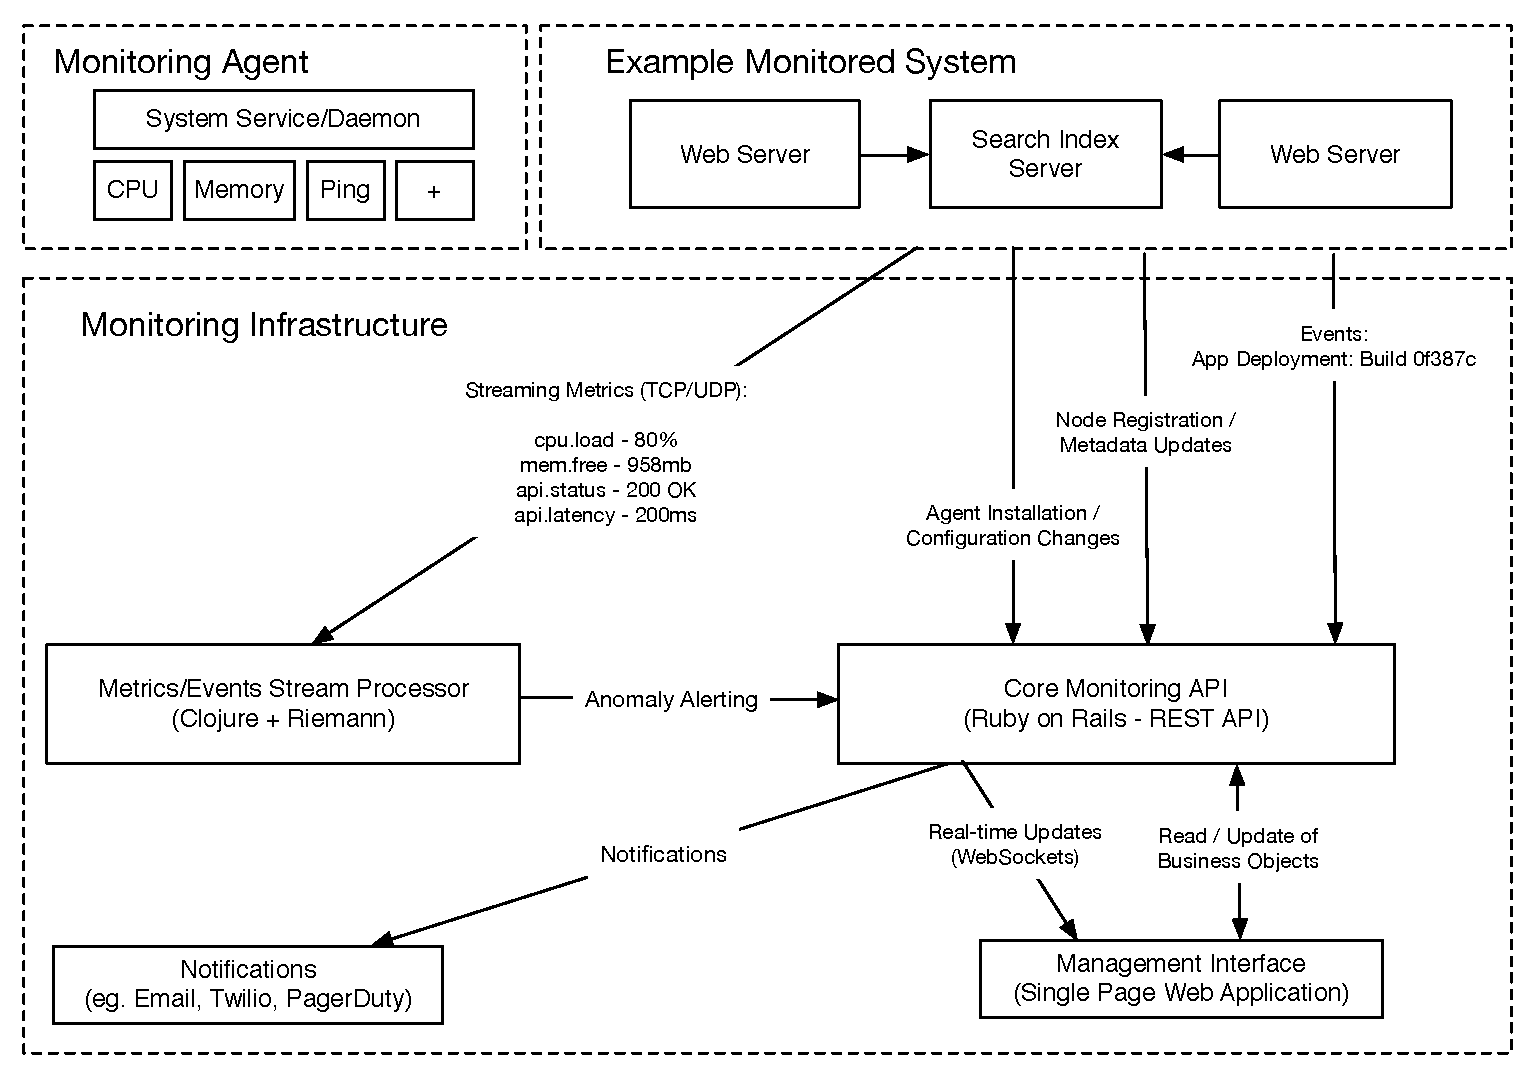
\includegraphics[scale=0.7]{architecture.pdf}
\end{landscape}

% \chapter{Implementation}
% \chapter{Professional Issues}
% \chapter{Evaluation}
% \chapter{Conclusion}

\printbibliography[title=References]
% \include{appendix}

\end{document}
